\subsection{Optics}

The optical train between the discharge lamp and the detector consists of two
plano-convex lenses, an interference filter, two linear polarisers, and a quarter-wave
plate. Each component is 50~mm in diameter.

\subsubsection*{Plano-Convex Lenses}

Two plano-convex lenses of focal length $f = 50$~mm are used to collimate the light
from the lamp and to focus it onto the detector. Plano-convex lenses minimise spherical
aberrations when the object and image distances differ greatly. The thin-lens equation
relates the object distance $d_o$, image distance $d_i$, and focal length $f$ :
\begin{equation}
    \frac{1}{d_o} + \frac{1}{d_i} = \frac{1}{f}
\end{equation}
Placing the first lens at $d_o \approx f = 50$~mm from the lamp bulb gives
$d_i \to \infty$, producing a collimated beam. The solid angle subtended by the
collimated beam at the absorption cell determines the fraction of lamp power collected :
\begin{equation}
    \Omega = \frac{\pi (D/2)^2}{d_o^2} = \frac{\pi D^2}{4d_o^2}
\end{equation}
where $D = 50$~mm is the lens diameter. The power delivered to the cell is then :
\begin{equation}
    P_{\text{cell}} = P_{\text{lamp}} \cdot \frac{\Omega}{4\pi}
                    = P_{\text{lamp}} \cdot \frac{D^2}{16\,d_o^2}
\end{equation}

\subsubsection*{Interference Filter}

The interference filter selects the 795~nm line while blocking the 780~nm line.
Its operation is based on thin-film multi-beam interference. For a cavity of optical
thickness $nd$, constructive interference (transmission peak) occurs at wavelengths
satisfying :
\begin{equation}
    2nd\cos\theta_r = m\lambda, \qquad m = 1,\,2,\,3,\ldots
\end{equation}
where $\theta_r$ is the refraction angle inside the cavity. When the filter is tilted by
an angle $\theta$ in air, Snell's law gives $\sin\theta_r = \sin\theta/n$, so the
transmission peak shifts to :
\begin{equation}
    \lambda(\theta) = \lambda_0\sqrt{1 - \frac{\sin^2\theta}{n^2}}
\end{equation}
where $\lambda_0$ is the normal-incidence peak wavelength and $n$ is the effective
refractive index of the filter. Since $\lambda(\theta) < \lambda_0$ for all $\theta > 0$,
tilting the filter \emph{blue-shifts} the transmission peak. The peak transmission of
the filter at 795~nm is approximately 0.80 (80\%).

\begin{figure}[h]
    \centering
    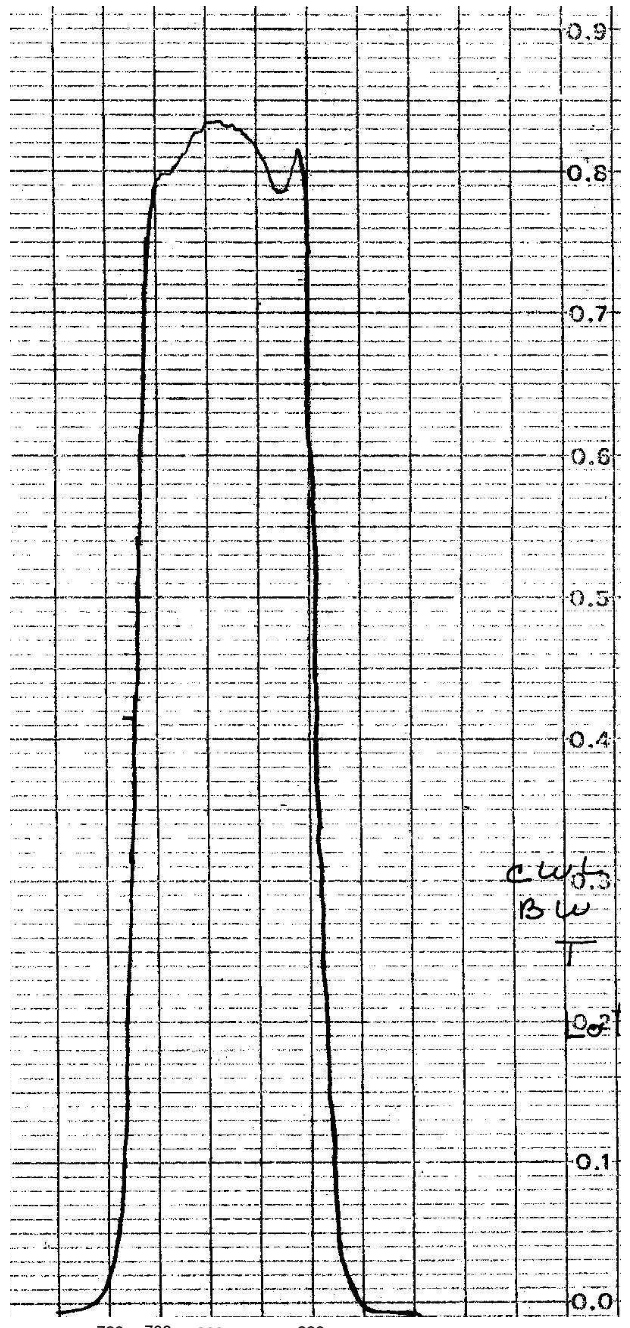
\includegraphics[width=0.55\textwidth]{figures/optics.png}
    \caption{Transmission characteristics of the interference filter.
             The peak near 795~nm selects the rubidium $D_1$ line.}
\end{figure}

\subsubsection*{Linear Polariser}

The linear polariser transmits only the component of the electric field along its
polarisation axis. For incident intensity $I_0$ with the polarisation axis at angle
$\phi$ to the incident field, Malus's law gives the transmitted intensity :
\begin{equation}
    I_t = I_0\cos^2\phi
\end{equation}
When two polarisers are crossed ($\phi = 90°$), the transmitted intensity vanishes
ideally. In practice, the extinction ratio $\epsilon$ is defined as :
\begin{equation}
    \epsilon = \frac{I_{\min}}{I_{\max}}
\end{equation}
Typical extinction ratios for the polarisers used are of order $10^{-3}$ to $10^{-4}$
(i.e.\ $\sim 2\%$ transmission at crossed configuration). The polarisation axis is
indicated by an alignment mark accurate to $\pm 5°$.

\begin{figure}[h]
    \centering
    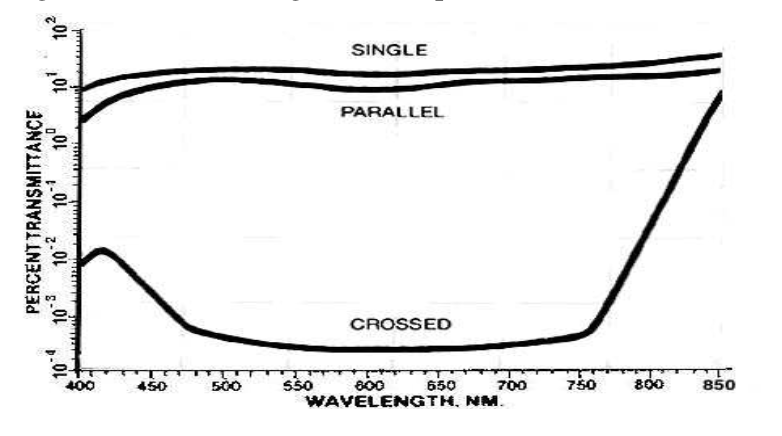
\includegraphics[width=0.55\textwidth]{figures/optics.2.png}
    \caption{Transmission characteristics of the linear polarisers (single, parallel,
             and crossed configurations).}
\end{figure}

\subsubsection*{Quarter-Wave Plate}

The quarter-wave plate converts linearly polarised light into circularly polarised
light. It has two optical axes — a fast axis and a slow axis — with refractive indices
$n_f$ and $n_s$ ($n_s > n_f$). The relative phase retardation accumulated over
physical thickness $t$ is :
\begin{equation}
    \Gamma = \frac{2\pi}{\lambda}(n_s - n_f)\,t
\end{equation}
For a quarter-wave plate, $\Gamma = \pi/2$, requiring :
\begin{equation}
    (n_s - n_f)\,t = \frac{\lambda}{4}
\end{equation}
The plate used has an optical thickness of $205 \pm 5$~nm, close to
$\lambda/4 = 795/4 \approx 198.75$~nm at the operating wavelength.

When linearly polarised light is incident at $45°$ to both axes, the electric field
components along the fast and slow axes are equal in amplitude :
\begin{equation}
    E_f = E_s = \frac{E_0}{\sqrt{2}}
\end{equation}
After passing through the plate, the slow component acquires a phase lag $\Gamma$
relative to the fast component. Writing the output field in Jones vector notation :
\begin{equation}
    \mathbf{E}_{\text{out}} = \frac{E_0}{\sqrt{2}}
    \begin{pmatrix} 1 \\ e^{i\Gamma} \end{pmatrix}
\end{equation}
For $\Gamma = \pi/2$ :
\begin{equation}
    \mathbf{E}_{\text{out}} = \frac{E_0}{\sqrt{2}}
    \begin{pmatrix} 1 \\ i \end{pmatrix}
\end{equation}
which represents \textbf{right circularly polarised} (RCP) light. The degree of
circular polarisation $P_c$ can be measured with a second linear polariser (analyser) :
\begin{equation}
    P_c = \sqrt{1 - \left(\frac{I_{\max} - I_{\min}}{I_{\max} + I_{\min}}\right)^2}
\end{equation}
For perfect circular polarisation $I_{\max} = I_{\min}$ and $P_c = 1$.

The optical thickness can be fine-tuned by tilting the plate by angle $\alpha$ about
the vertical axis. The retardation becomes :
\begin{equation}
    \Gamma(\alpha) = \frac{2\pi t}{\lambda}
    \left(\sqrt{n_s^2 - \sin^2\alpha} - \sqrt{n_f^2 - \sin^2\alpha}\right)
\end{equation}
Rotation about the slow axis increases $\Gamma$; rotation about the fast axis
decreases it.

\begin{figure}[h]
    \centering
    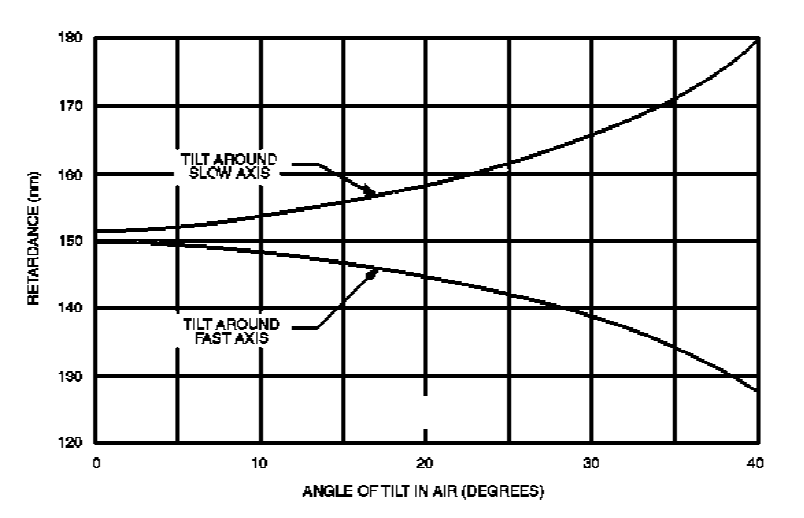
\includegraphics[width=0.55\textwidth]{figures/optics.3.png}
    \caption{Tilt tuning of the quarter-wave plate. Rotation about the slow (fast)
             axis increases (decreases) the retardation.}
\end{figure}

\subsubsection*{Complete Optical Train}

The components are arranged along the optical rail in the following order :
\begin{equation*}
    \text{Lamp} \;\to\;
    \text{Lens}_1 \;\to\;
    \text{IF} \;\to\;
    \text{LP} \;\to\;
    \text{QWP} \;\to\;
    \text{Cell} \;\to\;
    \text{Lens}_2 \;\to\;
    \text{Detector}
\end{equation*}
The centres of all components are set at a height of 3.5~inches above the optical rail.
The total transmission of the optical train (excluding cell absorption) is :
\begin{equation}
    T_{\text{total}} = T_{\text{IF}} \cdot T_{\text{LP}} \cdot T_{\text{QWP}}
    \cdot T_{L_1} \cdot T_{L_2}
\end{equation}
where each $T$ denotes the transmission coefficient of the corresponding element.